\chapter{Building High-Quality AI Agents}
\label{ch:building-agents}

\noindent
In early 2025, a developer tools startup demo'd their AI coding agent to a room of VCs. The agent received a prompt: ``Add pagination to the /users endpoint.'' It opened the right file, found the right function, wrote correct pagination logic, ran the tests, and committed the code. The room was impressed. The startup raised \$12 million.

Six months later, half their enterprise customers had churned. The agent that dazzled in a controlled demo failed catastrophically in real codebases: it would occasionally delete unrelated functions while editing a file. It couldn't handle monorepos with ambiguous import paths. When tests failed, it would sometimes ``fix'' them by making the tests less strict rather than fixing the code. One customer discovered the agent had silently disabled a rate limiter in production code because it was causing a test to flake.

The gap between a demo agent and a production agent is the same gap between a \code{SELECT * FROM users} and a production database: about three years of engineering. This chapter is about those three years.

AI agents represent the frontier of LLM application development. Unlike a simple LLM call that produces a single response, an agent can break down complex goals into steps, use tools to interact with external systems, maintain memory across interactions, and adapt its approach when initial strategies fail. Building agents that \emph{actually work}---reliably, safely, and cost-effectively---is among the hardest engineering challenges in the AI space.

\begin{figure}[htbp]
\centering
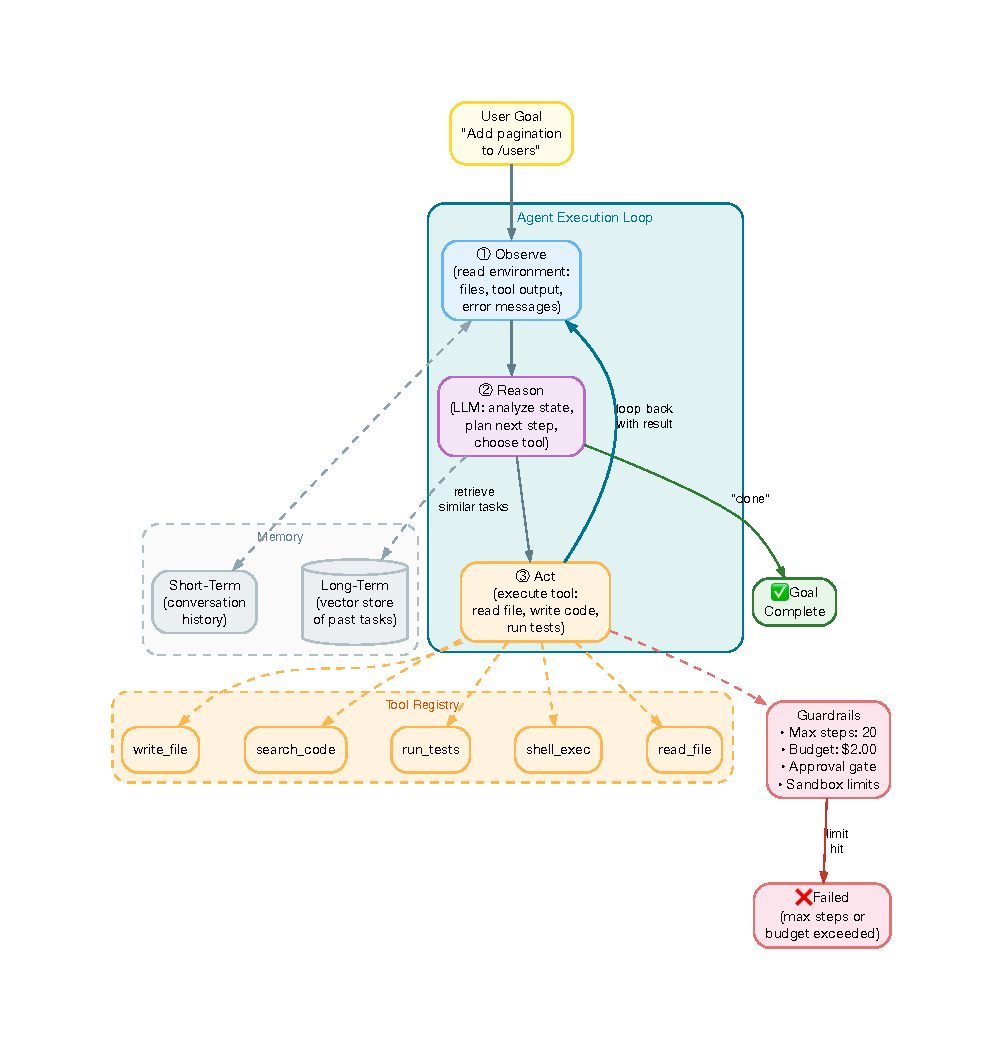
\includegraphics[width=\textwidth]{diagrams/compiled/ch12/agent-loop.pdf}
\caption{The core agent execution loop: observe $\to$ reason $\to$ act, with memory, tool registry, guardrails, and terminal states}
\label{fig:agent-loop}
\end{figure}


\section{What Makes an Agent}

An AI agent is a system that combines four capabilities:

\begin{enumerate}[leftmargin=*]
    \item \textbf{Perception}: The ability to observe the environment---reading files, parsing API responses, processing user input
    \item \textbf{Reasoning}: The ability to analyze observations and decide what to do next---an LLM serves as the reasoning engine
    \item \textbf{Action}: The ability to affect the environment---calling tools, writing files, executing code, sending messages
    \item \textbf{Memory}: The ability to maintain state across steps---conversation history, intermediate results, learned patterns
\end{enumerate}

The simplest possible agent is an LLM in a loop: the model receives a goal and a set of available tools, decides whether to call a tool or produce a final answer, and repeats until the task is complete. This simple loop---\emph{observe, reason, act}---is the kernel of every agent architecture. The differences between agent frameworks are in how they handle reasoning strategies, tool design, memory, error recovery, and multi-agent coordination.


\section{Agent Architectures}

Three dominant agent architecture patterns have emerged from both research and production experience. Each makes different trade-offs between interpretability, reliability, and cost. Figure~\ref{fig:agent-architectures} compares them side-by-side.

\begin{figure}[htbp]
\centering
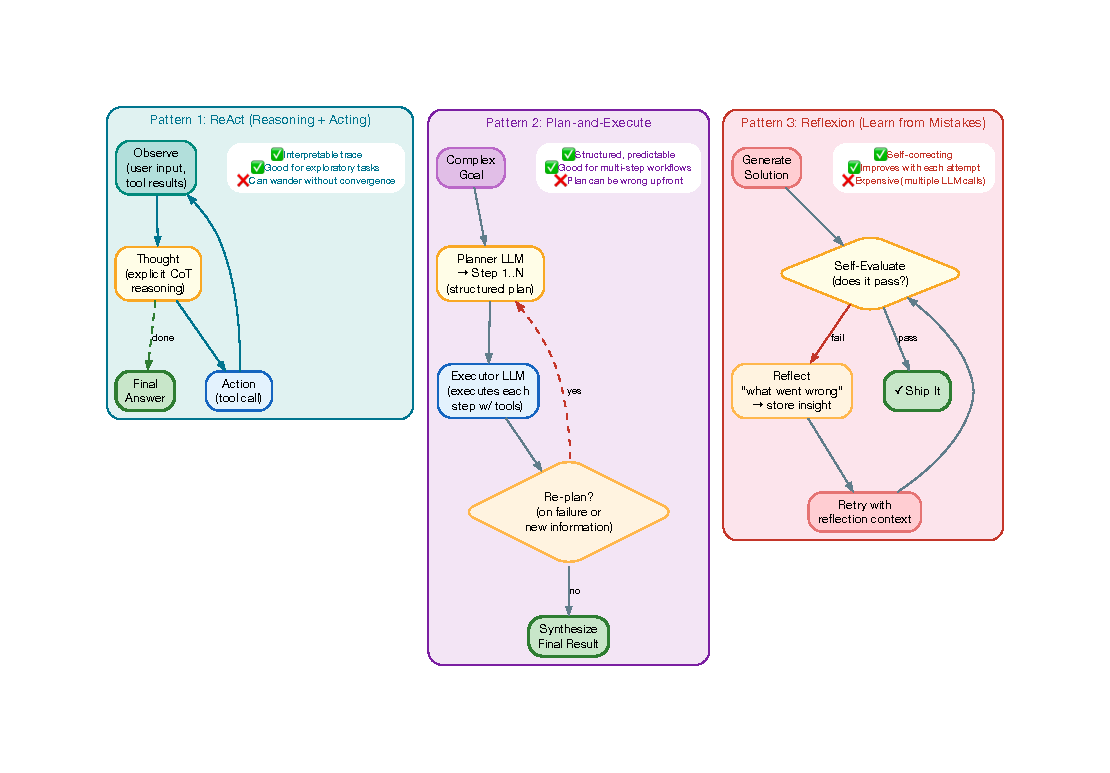
\includegraphics[width=\textwidth]{diagrams/compiled/ch12/agent-architectures.pdf}
\caption{Three agent architecture patterns compared: ReAct (interpretable, exploratory), Plan-and-Execute (structured, predictable), and Reflexion (self-correcting, expensive). Production systems often combine elements of all three.}
\label{fig:agent-architectures}
\end{figure}

\subsection{ReAct: Reasoning + Acting}

The \term{ReAct} pattern~\cite{yao2023react} interleaves reasoning (thinking about what to do) with acting (using tools). The model explicitly outputs its reasoning before each action, creating a transparent chain of thought. A typical ReAct trace looks like:

\begin{verbatim}
Thought: I need to find the users endpoint first.
Action:  search_files(query="def get_users", path="src/")
Observation: Found in src/api/users.py at line 47
Thought: Now I'll read that file to understand the current implementation.
Action:  read_file(path="src/api/users.py")
...
\end{verbatim}

The key advantage is \emph{interpretability}: you can read the agent's reasoning trace to understand why it took each action. This is invaluable for debugging and building trust. The disadvantage: ReAct agents can ``wander''---taking many exploratory steps without converging on a solution.

\subsection{Plan-and-Execute}

For complex, multi-step tasks, it's often better to plan first, then execute. The \term{Plan-and-Execute} pattern uses a \emph{planner LLM} to decompose the goal into a structured list of steps, then an \emph{executor LLM} works through each step sequentially. Crucially, the agent can \emph{re-plan} when a step fails or produces unexpected results.

This pattern excels at tasks with clear decomposition (``migrate this API from REST to gRPC,'' ``set up CI/CD for this repo''), but can struggle when the initial plan is fundamentally wrong---the agent may waste many steps before triggering a re-plan.

\subsection{Reflexion: Learning from Mistakes}

\term{Reflexion} adds a self-evaluation step after each attempt. If the agent's output doesn't meet quality standards, it reflects on what went wrong and tries again with the reflection as additional context. This is particularly effective for code generation, where the agent can run tests, see failures, and iteratively fix its solution.

The cost trade-off is real: a reflexion agent may make 3--5 LLM calls to solve a task that a ReAct agent attempts in one pass. But for high-stakes tasks (production code changes, customer-facing content), the additional cost is often justified by higher success rates.

\begin{keytakeaway}
In practice, production agents often combine elements of all three patterns: plan first (Plan-and-Execute), reason transparently at each step (ReAct), and retry with reflection when things fail (Reflexion). The architecture is not a religion---it's a set of tools to compose.
\end{keytakeaway}


\section{The Evolution of Reasoning Paradigms}

The patterns described above---ReAct, Plan-and-Execute, Reflexion---did not emerge in isolation. They are part of a rapid evolution of reasoning paradigms that began with Chain-of-Thought prompting in 2022 and has since produced reasoning models, multi-agent systems, and flow engineering. Understanding this lineage is essential for choosing the right approach and anticipating what comes next.

Figure~\ref{fig:reasoning-paradigms} traces the full evolution.

\begin{figure}[htbp]
\centering
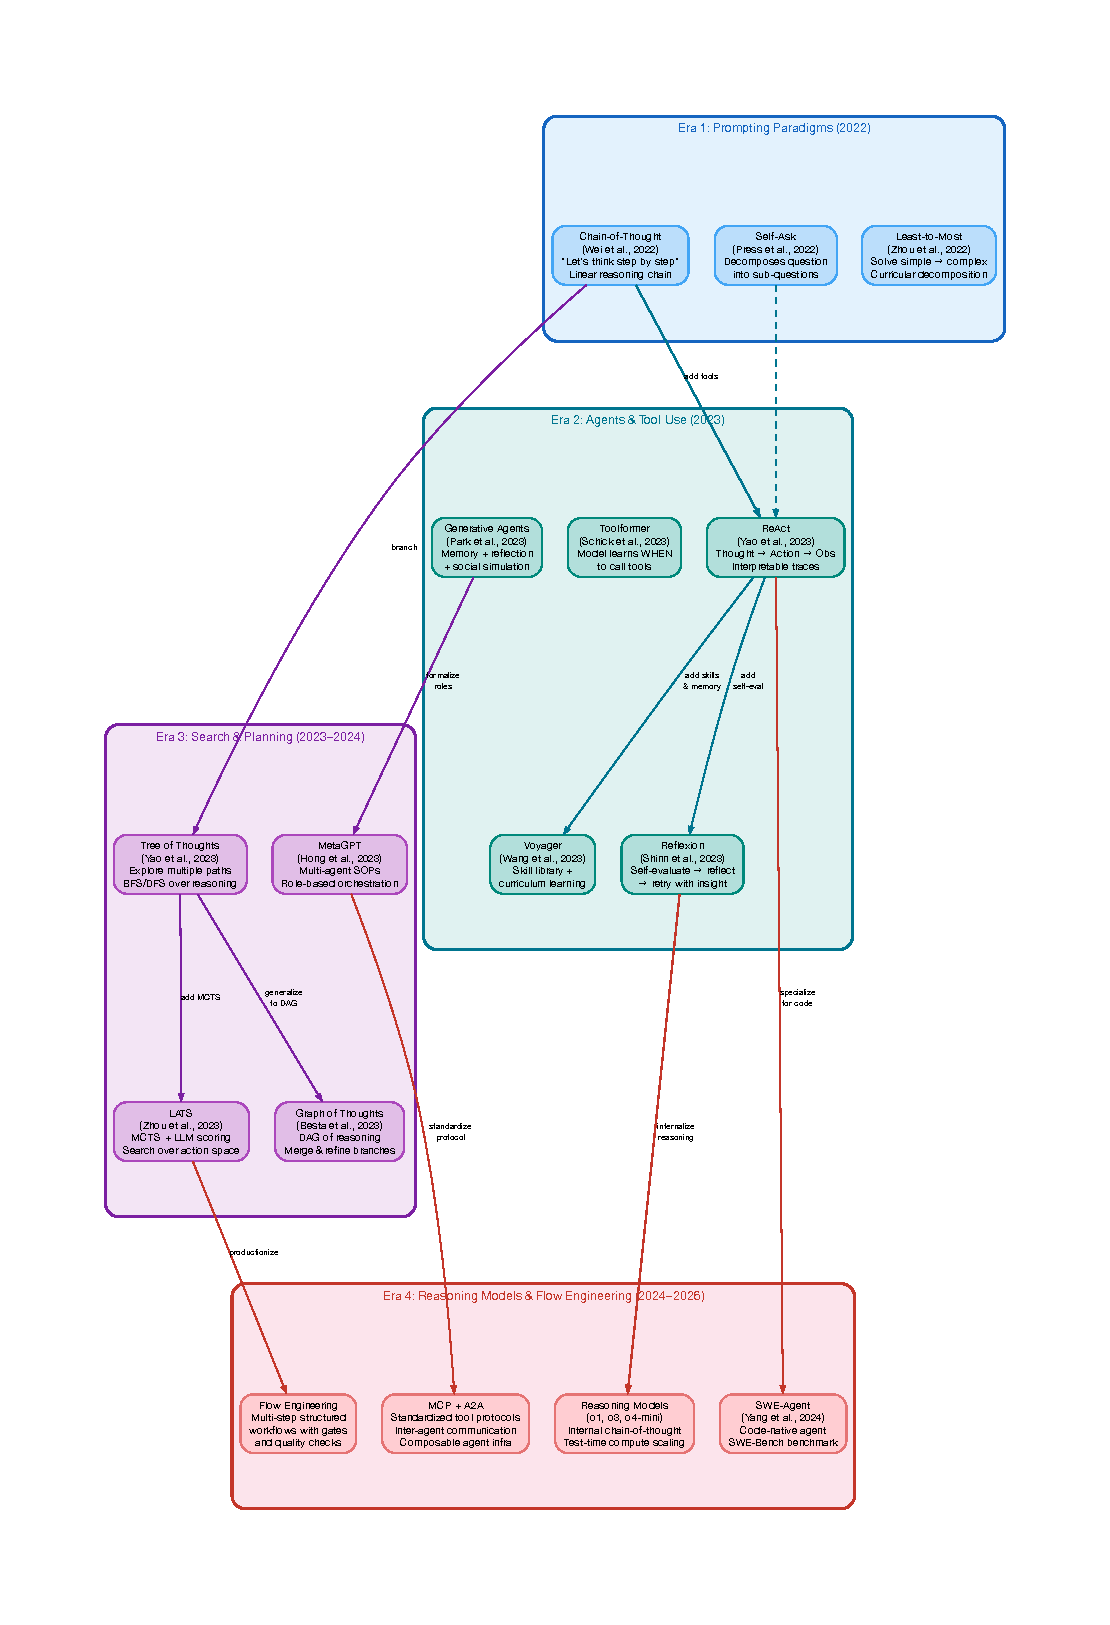
\includegraphics[width=\textwidth]{diagrams/compiled/ch12/reasoning-paradigms.pdf}
\caption{Four eras of reasoning paradigms: from Chain-of-Thought prompting (2022) through agents and tool use (2023), search and planning (2023--2024), to reasoning models and flow engineering (2024--2026). Arrows show evolutionary lineage between patterns.}
\label{fig:reasoning-paradigms}
\end{figure}

\subsection{Era 1: Prompting Paradigms (2022)}

The revolution began with a deceptively simple insight: if you ask an LLM to ``think step by step,'' it produces dramatically better answers.

\textbf{Chain-of-Thought (CoT)} (Wei et al., 2022) showed that adding ``Let's think step by step'' to a prompt---or providing worked examples with intermediate reasoning---improved GPT-3's performance on math and logic tasks from near-random to competitive with fine-tuned models. The mechanism: CoT forces the model to decompose problems into intermediate steps, and each step's output provides context for the next.

\textbf{Self-Ask} (Press et al., 2022) took this further: the model explicitly asks itself follow-up questions (``But wait, do I know what the capital of Burkina Faso is?''), answers them, and then continues. This makes the decomposition structure explicit and composable.

\textbf{Least-to-Most} (Zhou et al., 2022) introduced curriculum-style decomposition: break a hard problem into a sequence of progressively harder sub-problems, solve them in order, and use each answer as context for the next. This pattern is particularly effective for complex reasoning that builds on itself.

The engineering lesson from Era 1: \emph{how you ask matters as much as what you ask}. Prompting strategy is an engineering discipline, not a creative writing exercise.

\subsection{Era 2: Agents and Tool Use (2023)}

Era 1's paradigms were stateless---the model reasoned within a single context window with no ability to interact with the outside world. Era 2 added tools, memory, and persistent state.

\textbf{ReAct} (Yao et al., 2023) combined Chain-of-Thought with tool use: the model outputs a \emph{Thought} (reasoning), an \emph{Action} (tool call), and observes the result. This interleaving of reasoning and acting produced the first agents that could browse the web, query databases, and execute code as part of their reasoning process.

\textbf{Toolformer} (Schick et al., 2023) took a different approach: instead of prompting the model to use tools, they fine-tuned it to \emph{learn when to call tools}. The model learned to insert API calls (calculator, search, translator) into its generation when they would improve the output. This was an early signal that tool use could be internalized rather than orchestrated externally.

\textbf{Reflexion} (Shinn et al., 2023) added the self-improvement loop: after each attempt, the agent evaluates its output, generates a natural language reflection on what went wrong, and uses that reflection as additional context for the next attempt. On coding benchmarks (HumanEval), Reflexion improved first-pass accuracy from 67\% to 91\% by iterating.

\textbf{Voyager} (Wang et al., 2023) introduced the concept of a \emph{skill library}: an agent playing Minecraft would learn new skills (``how to craft a diamond pickaxe''), store them as reusable code functions, and compose them for novel tasks. This is the agent equivalent of learning---converting slow exploration into fast execution through procedural memory.

\textbf{Generative Agents} (Park et al., 2023) created a small simulated town where 25 LLM-powered agents lived, worked, and socialized. The key innovation was the memory architecture: agents stored experiences, reflected on them periodically (``What did I learn today?''), and used those reflections to plan future actions. This demonstrated that memory + reflection produces emergent social behaviors without explicit programming.

\subsection{Era 3: Search and Planning (2023--2024)}

Chain-of-Thought produces a single linear chain of reasoning. But many problems have multiple valid approaches, and the first approach may be wrong. Era 3 explored structured search over the space of possible reasoning paths.

\textbf{Tree of Thoughts (ToT)} (Yao et al., 2023) treats each reasoning step as a node in a tree. At each step, the model generates multiple candidate continuations, evaluates them, and selects the most promising path---essentially applying BFS or DFS to reasoning. This dramatically improved performance on tasks requiring exploration (crossword puzzles, creative writing, planning), at the cost of $3$--$5\times$ more LLM calls.

\textbf{Graph of Thoughts (GoT)} (Besta et al., 2023) generalized trees to directed acyclic graphs: different reasoning branches can be \emph{merged} and \emph{refined}. For example, two branches might independently discover relevant facts that, combined, produce a better answer than either alone.

\textbf{LATS (Language Agent Tree Search)} (Zhou et al., 2023) combined tree search with Monte Carlo Tree Search (MCTS)---the same algorithm behind AlphaGo. The agent uses an LLM to evaluate states, select actions, and backpropagate rewards through the search tree. On WebShop and HotPotQA benchmarks, LATS outperformed ReAct by $22$--$45\%$.

\textbf{MetaGPT} (Hong et al., 2023) brought software engineering practices to multi-agent systems: agents are assigned roles (product manager, architect, engineer, QA), follow standard operating procedures (SOPs), and produce structured artifacts at each stage. The insight: multi-agent coordination fails without process---the same lesson that human software teams learned decades ago.

\subsection{Era 4: Reasoning Models and Flow Engineering (2024--2026)}

The most recent era has been shaped by two converging trends: the internalization of reasoning into model weights, and the productionization of agent workflows.

\textbf{Reasoning models} (OpenAI o1, o3, o4-mini) represent a paradigm shift: instead of external Chain-of-Thought prompting, the model performs extended internal reasoning before generating a response. The model uses ``test-time compute scaling''---spending more compute on harder problems---to achieve dramatically better results on math, science, and coding benchmarks. The engineering implication: for complex reasoning tasks, you can now trade a sophisticated agent architecture for a single call to a reasoning model, at the cost of higher latency and token usage.

\textbf{SWE-Agent} (Yang et al., 2024) demonstrated that agent architecture matters enormously for coding tasks. By designing a code-native agent interface (custom file viewer, search tools, edit commands), SWE-Agent achieved state-of-the-art performance on SWE-Bench, solving real GitHub issues end-to-end. The lesson: generic agent frameworks underperform domain-specialized agent designs.

\textbf{Flow Engineering} has emerged as the production-grade approach to agent systems. Instead of a single autonomous agent, flow engineering breaks a task into a structured, multi-step workflow with explicit quality gates between stages. Each stage may use a different model, different prompt, and different evaluation criteria. Stages can be retried independently. The workflow is version-controlled, tested, and monitored like any other software system.

\textbf{MCP and A2A protocols} (covered in the next section) standardized the infrastructure layer, making it possible to compose agents from modular, interchangeable components rather than building monolithic systems.

\begin{tipbox}[Choosing the Right Paradigm]
Use this decision framework:
\begin{itemize}[leftmargin=*]
    \item \textbf{Simple Q\&A or classification}: Direct prompting or CoT. No agent needed.
    \item \textbf{Tasks requiring external data}: ReAct with tools. The bread-and-butter agent pattern.
    \item \textbf{Multi-step workflows with known structure}: Plan-and-Execute or Flow Engineering. Predictable, testable.
    \item \textbf{Tasks where quality matters more than cost}: Reflexion or Tree of Thoughts. Multiple attempts with self-evaluation.
    \item \textbf{Hard reasoning problems}: Reasoning models (o4-mini for cost, o3 for quality). Single call, high compute.
    \item \textbf{Tasks requiring multiple expertise areas}: Multi-agent with A2A. Use only when single-agent demonstrably fails.
\end{itemize}
\end{tipbox}

\section{Tool Use and the MCP Ecosystem}

Tools are the agent's hands---they let it interact with the real world. In 2024--2025, the agent ecosystem converged around a standard protocol for tool integration: the \textbf{Model Context Protocol (MCP)}. Understanding MCP, Skills, and A2A is essential for building modern agents.

\subsection{The Model Context Protocol (MCP)}

Before MCP, every agent framework had its own way of defining and calling tools. If you built a database tool for LangChain, it didn't work in CrewAI or AutoGen. MCP, originally introduced by Anthropic and now an industry-wide standard, provides a \emph{universal protocol} for connecting AI agents to tools and data sources.

\begin{figure}[htbp]
\centering
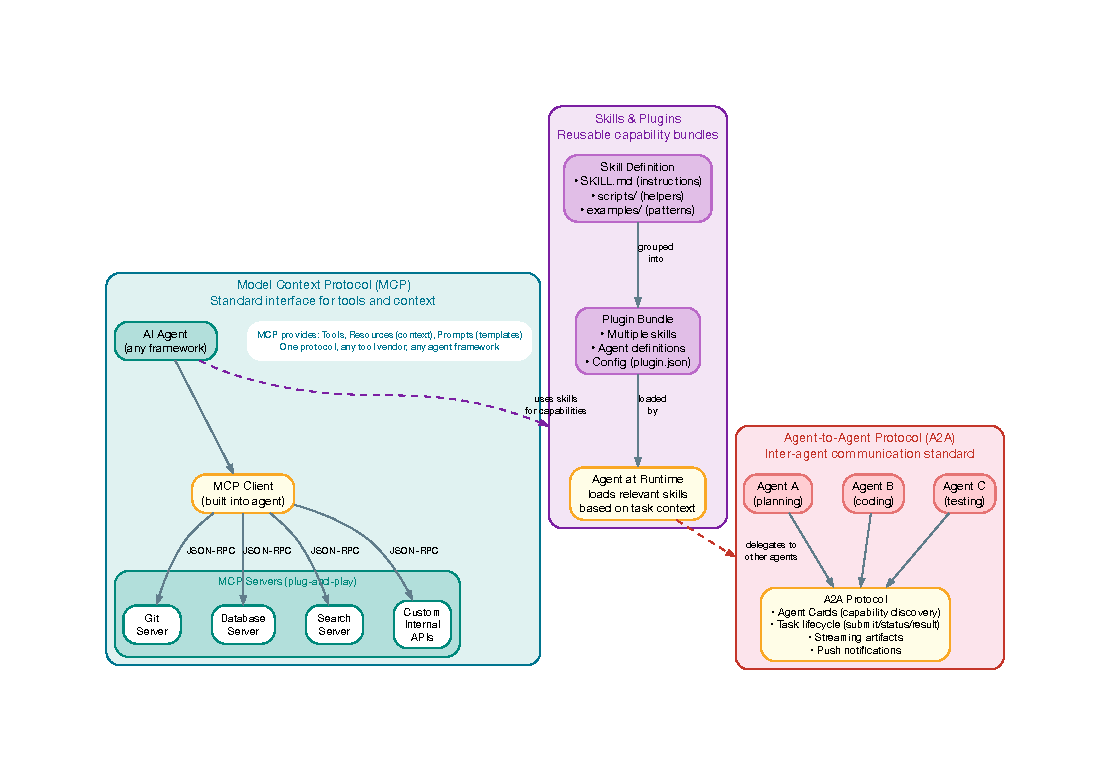
\includegraphics[width=\textwidth]{diagrams/compiled/ch12/mcp-a2a-skills.pdf}
\caption{The modern agent ecosystem: MCP provides a standard tool interface, Skills bundle reusable capabilities, and A2A enables inter-agent communication. Together, they form the composable infrastructure layer.}
\label{fig:mcp-a2a-skills}
\end{figure}

MCP uses a client-server architecture over JSON-RPC:

\begin{itemize}[leftmargin=*]
    \item \textbf{MCP Servers} expose capabilities---a Git server provides commit, diff, and search tools; a database server provides query and schema inspection tools; a search server provides web or internal document search.
    \item \textbf{MCP Clients} (built into the agent) discover and call these servers. The agent's tool registry is populated dynamically from whatever MCP servers are configured.
    \item \textbf{Three primitives}: Tools (functions the agent can call), Resources (contextual data the agent can read), and Prompts (reusable prompt templates).
\end{itemize}

The key engineering insight: MCP separates \emph{tool implementation} from \emph{agent implementation}. You can build an MCP server for your internal APIs once and it works with any MCP-compatible agent---Claude, Gemini, GPT-5.5, or your own custom agent.

\subsection{Skills and Plugins}

MCP servers provide individual tools. \textbf{Skills} provide higher-level capabilities---a bundle of instructions, scripts, and examples that teach an agent how to perform a complex task. A skill might include:

\begin{itemize}[leftmargin=*]
    \item A \code{SKILL.md} file with detailed instructions (e.g., ``how to deploy a Firebase app'')
    \item Helper scripts that the agent can execute
    \item Example patterns and reference implementations
    \item The MCP servers required for the skill to function
\end{itemize}

Skills are grouped into \textbf{Plugins}---bundles of related skills, agent definitions, and configuration. This composable architecture means an agent's capabilities are modular: you can add Firebase support by installing a Firebase plugin, or add bioinformatics capabilities by installing a science plugin. The agent loads the relevant skills at runtime based on the task context.

\begin{tipbox}[Skill Design Principle]
The best skills follow the ``recipe'' pattern: they contain the \emph{judgment calls} and \emph{decision criteria} that a senior engineer would know, not just the API calls. A good Firebase deployment skill doesn't just list CLI commands---it tells the agent when to use App Hosting vs.\ static Hosting, how to handle environment variables, and what to check before deploying.
\end{tipbox}

\subsection{Agent-to-Agent Protocol (A2A)}

For complex tasks that exceed a single agent's capabilities, \textbf{A2A} (Agent-to-Agent) provides a standard for inter-agent communication, developed by Google and now adopted broadly. Key concepts:

\begin{itemize}[leftmargin=*]
    \item \textbf{Agent Cards}: A JSON manifest declaring an agent's capabilities, skills, and constraints. Like an API spec, but for agents.
    \item \textbf{Task Lifecycle}: A standard protocol for submitting tasks, checking status, streaming partial results, and receiving completion notifications.
    \item \textbf{Artifact Exchange}: Agents can pass structured artifacts (code, documents, test results) as first-class objects.
    \item \textbf{Push Notifications}: Long-running agent tasks can notify the requester asynchronously rather than requiring polling.
\end{itemize}

The combination of MCP (tool access) + Skills (capability bundles) + A2A (agent collaboration) forms the infrastructure layer that makes multi-agent systems practical at scale.


\subsection{Tool Design Principles}

Whether you expose tools via MCP or directly, the design principles are the same:

\begin{enumerate}[leftmargin=*]
    \item \textbf{Clear, descriptive names}: \code{search\_documentation} is better than \code{search}. The LLM uses the name to decide when to use the tool.
    
    \item \textbf{Excellent docstrings}: The tool's description is part of the prompt. A vague description leads to misuse.
    
    \item \textbf{Atomic operations}: Each tool should do one thing well. Don't combine ``search and summarize'' into a single tool.
    
    \item \textbf{Structured inputs and outputs}: Use typed parameters with clear constraints. Return structured data, not free-form text.
    
    \item \textbf{Graceful error handling}: Tools should never crash. Return clear error messages that help the agent recover.
    
    \item \textbf{Idempotent where possible}: If the agent retries a tool call, it shouldn't cause duplicate side effects.
\end{enumerate}


\section{Memory Systems}

Agents need memory at multiple timescales. Figure~\ref{fig:memory-tiers} shows the three tiers of agent memory and how they interact.

\begin{figure}[htbp]
\centering
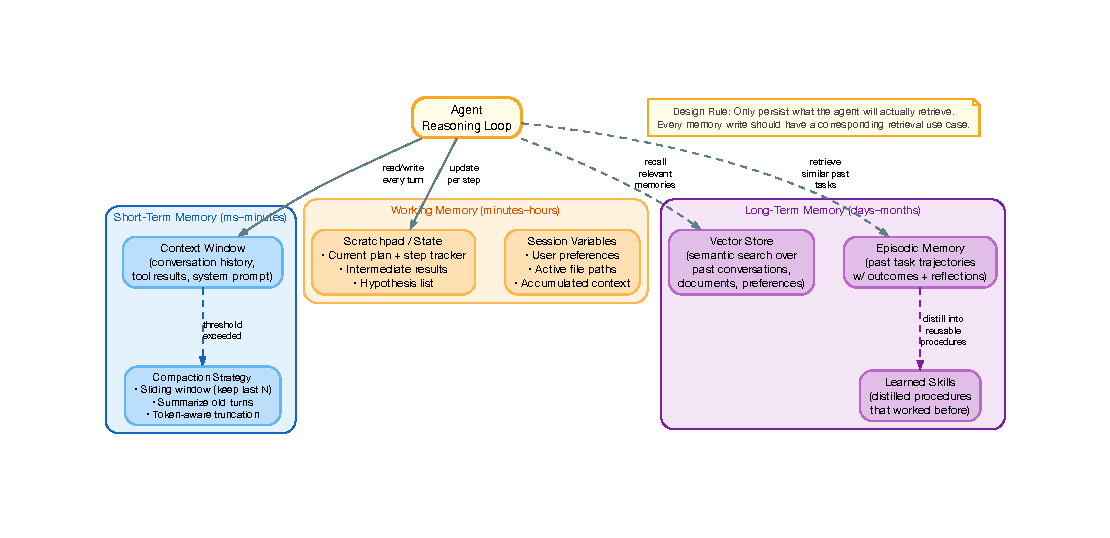
\includegraphics[width=\textwidth]{diagrams/compiled/ch12/memory-tiers.pdf}
\caption{Three tiers of agent memory: short-term (context window), working memory (session state), and long-term (persistent vector store with episodic recall and learned skills)}
\label{fig:memory-tiers}
\end{figure}

\subsection{Short-Term Memory: The Context Window}

The simplest form of memory: the LLM's context window. Every message, tool result, and observation from the current session is included in the prompt. The challenge: context windows have finite size, and performance degrades as the context grows. Even models with 1M+ token context windows show diminished recall for information in the ``lost middle'' of very long contexts.

Three compaction strategies:
\begin{itemize}[leftmargin=*]
    \item \textbf{Sliding window}: Keep only the last N messages. Simple but loses early context.
    \item \textbf{Summarization}: Periodically summarize older messages into a compact paragraph. Preserves key information but loses detail.
    \item \textbf{Token-aware truncation}: Monitor token count and compact when approaching threshold. Keep the system prompt, first user message, and most recent messages intact.
\end{itemize}

\subsection{Working Memory: Session State}

Beyond the raw context window, agents benefit from structured working memory:

\begin{itemize}[leftmargin=*]
    \item \textbf{Plan tracker}: The current plan with step status (pending/running/done/failed)
    \item \textbf{Intermediate results}: Partial outputs that downstream steps depend on
    \item \textbf{Hypothesis list}: For debugging agents, a running list of hypotheses being tested
    \item \textbf{Session variables}: User preferences, active file paths, accumulated context
\end{itemize}

This working memory is typically stored as a structured data object that the agent reads and updates at each step, separate from the raw conversation history.

\subsection{Long-Term Memory: Persistent Knowledge}

For information that should persist across sessions, agents use vector databases to store and retrieve relevant past experiences. Three types of long-term memory have proven valuable:

\textbf{1. Semantic memory} --- General knowledge stored as embeddings. Past conversations, documents, and user preferences are embedded and retrieved via semantic similarity search.

\textbf{2. Episodic memory} --- Records of completed tasks with their trajectories and outcomes. When facing a new task, the agent retrieves similar past tasks and uses their trajectories as in-context examples. This is particularly powerful for tasks the agent has solved before---it can replay a known-good strategy rather than exploring from scratch.

\textbf{3. Learned skills} --- Procedures distilled from successful task completions. If the agent has deployed a Firebase app ten times, it can distill the common steps into a reusable procedure that skips the exploration phase entirely. This is the agent equivalent of converting slow System 2 reasoning into fast System 1 pattern matching.

\begin{cautionbox}[Memory Design Rule]
Only persist what the agent will actually retrieve. Every memory write should have a corresponding retrieval use case. Agents that store everything create a ``memory dump'' that degrades retrieval quality over time.
\end{cautionbox}


\section{Multi-Agent Systems}

For complex tasks, a single agent may not be sufficient. Multi-agent systems decompose problems across specialized agents that collaborate.

\subsection{Orchestration Patterns}

\begin{figure}[htbp]
\centering
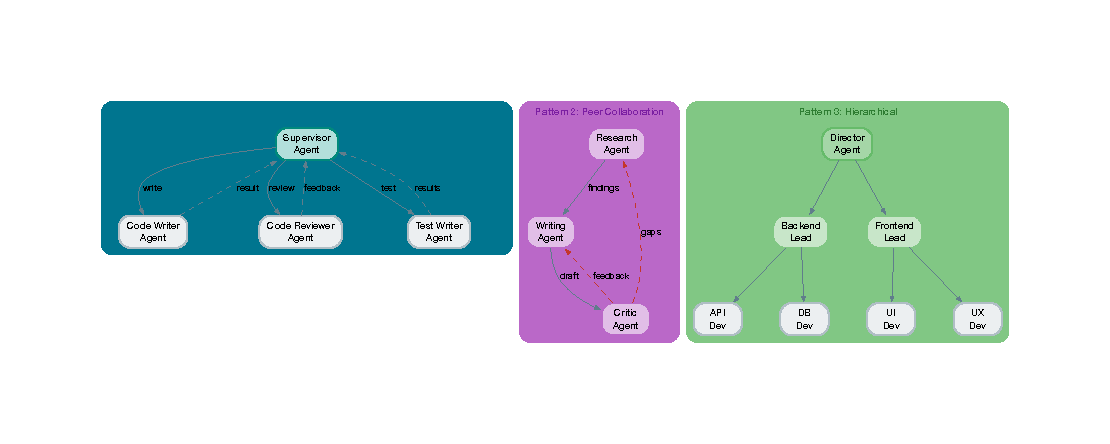
\includegraphics[width=\textwidth]{diagrams/compiled/ch12/multi-agent.pdf}
\caption{Multi-agent orchestration patterns: supervisor (most common), peer collaboration (creative tasks), and hierarchical delegation (complex, multi-day tasks)}
\label{fig:multi-agent}
\end{figure}

Three main patterns have emerged:

\textbf{1. Supervisor pattern}: A ``manager'' agent delegates tasks to specialized worker agents and synthesizes their results. The supervisor decides which specialists to involve, what subtask each should handle, and how to combine results. This is the most common pattern for well-defined workflows.

\textbf{2. Peer collaboration}: Agents communicate as peers, each contributing their expertise. One agent might write code while another reviews it. A third might write tests. Agents exchange artifacts (code, reviews, test results) via A2A protocol. This works well for creative tasks where the solution space is uncertain.

\textbf{3. Hierarchical delegation}: Multiple layers of management, where high-level agents delegate to mid-level agents, who further decompose and delegate. Used for very complex, multi-day tasks like large codebase migrations or comprehensive research projects.

\begin{tipbox}[Start Simple]
Most teams should start with a single-agent ReAct loop and only introduce multi-agent systems when the single agent demonstrably fails. Multi-agent systems add significant complexity in debugging, cost control, and failure mode analysis.
\end{tipbox}


\section{Guardrails and Safety}

Autonomous agents can cause real harm if not properly constrained. Safety engineering for agents is not optional---it's a prerequisite for production deployment.

\begin{figure}[htbp]
\centering
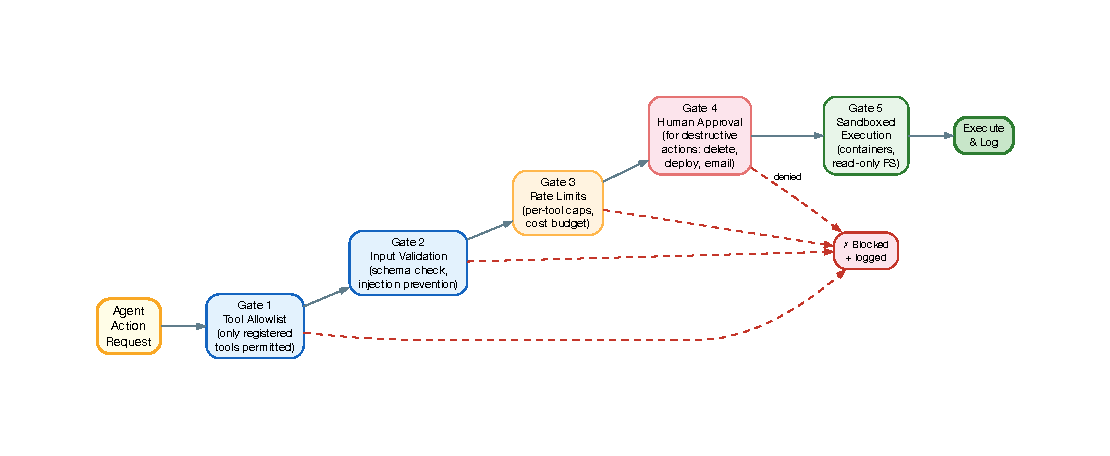
\includegraphics[width=\textwidth]{diagrams/compiled/ch12/agent-guardrails.pdf}
\caption{The five-gate guardrail pipeline: every agent action passes through allowlist check, input validation, rate limiting, human approval (for destructive actions), and sandboxed execution before executing}
\label{fig:agent-guardrails}
\end{figure}

\subsection{The Five Gates}

Every tool call from an agent should pass through a layered guardrail pipeline:

\begin{enumerate}[leftmargin=*]
    \item \textbf{Tool allowlist}: Only explicitly registered tools can be called. The agent cannot dynamically discover or invoke arbitrary functions.
    
    \item \textbf{Input validation}: Tool arguments are validated against a schema before execution. This prevents prompt injection attacks where the LLM is tricked into passing malicious arguments.
    
    \item \textbf{Rate limiting}: Per-tool call caps and per-session cost budgets. An agent that enters an infinite loop should hit a rate limit before it exhausts your API budget.
    
    \item \textbf{Human approval}: Destructive actions (deleting files, deploying to production, sending emails, modifying databases) require explicit human approval. The agent presents the proposed action and waits for confirmation.
    
    \item \textbf{Sandboxed execution}: Tools execute in isolated environments---containers, restricted filesystems, network-limited sandboxes. Even if the agent's judgment is wrong, the blast radius is contained.
\end{enumerate}

\subsection{Cost Control}

Agent costs can spiral quickly. A reasoning-heavy agent using GPT-5.5 might spend \$5--10 per complex task. A multi-agent system might multiply that by 3--5x. Production agent systems need:

\begin{itemize}[leftmargin=*]
    \item \textbf{Per-task cost budgets}: Hard caps on total spend per task execution
    \item \textbf{Step limits}: Maximum number of reasoning steps (typically 20--50)
    \item \textbf{Model tier routing}: Route simple sub-tasks to cheaper models (see Chapter~\ref{ch:app-architecture})
    \item \textbf{Cost observability}: Real-time dashboards showing cost per task, per agent, per user
\end{itemize}

\begin{keytakeaway}
Building production-quality agents requires much more than chaining LLM calls with tools. The engineering challenges---memory management, error recovery, safety guardrails, cost control, and multi-agent coordination---are where most of the complexity lives. Start simple (a single-agent ReAct loop), validate that it works, then add complexity only as needed. Use MCP for tool integration, Skills for capability composition, and A2A when you truly need multi-agent collaboration.
\end{keytakeaway}

\section{Chapter Summary}

Building high-quality AI agents requires mastering four capabilities and three engineering disciplines:

\textbf{Four capabilities}: perception, reasoning, action, and memory.

\textbf{Three engineering disciplines}:
\begin{enumerate}[leftmargin=*]
    \item \textbf{Architecture}: Choose the right pattern (ReAct, Plan-and-Execute, Reflexion) for your task's complexity
    \item \textbf{Tool ecosystem}: Use MCP for standard tool integration, Skills for capability composition, and A2A for multi-agent communication. Well-designed tools are the single biggest leverage point.
    \item \textbf{Safety engineering}: The five-gate guardrail pipeline (allowlist, validation, rate limiting, approval, sandboxing) is not optional for production agents
\end{enumerate}
